\documentclass[twocolumn,12pt]{article}
\usepackage[spanish]{babel}
\title{\textbf{{\LARGE ANÁLISIS DE PRODUCTOS}}}
\author{{\Large Angélica María Martínez Céspedes} \\ {\large Universidad de La Habana}\\{\small Facultad de Matemática y Computación}} 
\usepackage{graphicx}
\usepackage{hyperref}
\usepackage{amsmath}


\begin{document}
	
	
\twocolumn[\begin{@twocolumnfalse}
\maketitle
\begin{abstract}
En el siguiente informe se expone detalladamente el análisis realizado de algunos productos como: la cerveza, la cebolla y los refrescos ,con el objetivo de identificar patrones, tendencias y relaciones  en los datos. Se utilizaron métodos estadísticos para estudiar  los datos, se generaron gráficos y tablas para mostrar los resultados de dichos análisis y llegar a conclusiones efectivas.Los hallazgos clave del análisis incluyen la varianción del precio de la cerveza , la cebolla y los refrescos y las hipótesis con sostén del por qué, además se examinaron otros aspectos influyentes para la caracterización de cada producto desde su precio, cantidad, locazación, entre otros aspectos.

\textit{\underline{Palabras Claves: Análisis de Datos,Productos,Cerveza,Cebolla,Refrescos.}}
\end{abstract}
\end{@twocolumnfalse}
]

\section{{\LARGE \underline{Introducción}}}

\begin{center}
	"Travesía Inesperada"
\end{center}
           
La Universidad de La Habana , especifícamente la Facultad de Matemática y Computación conocida como MatCom llevo a cabo la creación de una nueva carrera:"Ciencia de datos" , más conocida como Data Science , la cual como podrán deducir por su nombre trata sobre la extracción de información explotable a partir de datos brutos , es decir , es un campo multidisciplinar que tiene como objetivo principal identificar tendencias , conceptos , motivos , prácticas , conexiones y correlaciones en las grandes series de datos , parece interesante cierto ? pues resulta más interesante la investigación realizada por uno los estudiantes de primero de la carrera , quien realiza un análisis acerca de los diferentes precios de algunos productos de mercado como la cerveza , la cebolla y los refrescos en un determinado municipio , teniendo en cuenta además otros aspectos de dichos productos para llevar a cabo su estudio .Cabe destacar que para el proceso de extración de estos datos fue necesario dirigirse hasta cada uno de los puntos de venta donde se ofertaban dichas mercancías , acción que implicó un extenso recorrido atestado de situaciones inesperadas que se comentarán más adelante .Este tipo de análisis posee un nombre concreto : "periodismo de datos" , en la ciencia de datos el periodismo de datos se utiliza para contar historias basadas en datos y para comunicar los resultados de análisis complejos a un público más amplio , también se utiliza para descubrir patrones y tendencias en los datos que pueden ser útiles para la investigación científica .Luego de haber entrado un poco en contexto sobre el objetivo de este estudio para la compresión del lector , comienza la travesía ...\\

En un inicio a cada estudiante de la carrera se le otorgó un municipio diferente para realizar las observaciones , pero se acordó de manera inteligente entre todos los estudiantes crear equipos para salir en la búsqueda de la información y poder sacar provecho de ello , pues tendrían un campo más amplio de referencias para establecer comparaciones entre los precios de los productos y llegar a una conclusión .Cuatro estudiantes amigos decieron formar un equipo en conjunto , integrado por dos hembras y dos varones , y así recorrer juntos los cuatro municipios otorgados a cada uno de ellos : el Cerro , Centro Habana , la Habana Vieja y Guanabacoa .En la semana de receso , especifícamente un martes tres de ellos salieron en busca de capturar los datos , faltaba un integrante pues se encontraba en provincia y no regresaba hasta el miércoles , los otros tres decidieron empezar por el municipio de la Habana Vieja puesto que hipotéticamente es un territorio reducido y considerado una de las zonas más turísticas de La Habana  debido a la restauración y conservación de su arquitectura colonial , por ende cuenta con una variada oferta cultural y gastronómica , que va desde restaurantes de todo tipo , bares, cantinas , cafeterías y famosos centros nocturnos .El punto de encuentro y partida fue en la Embajada de Espana .El recorrido comenzó en el conocido callejón de los barberos y avanzaron sucesivamente completando todo el municipio , el mismo día caminaron parte del municipio Centro Habana hasta que la oscuridad y el cansancio dieron por concluido el trayecto .Al otro día se incorporo el integrante faltante del equipo y los cuatro universitarios terminaron de recorrer el municipio Centro Habana y partieron hacia el municipio Cerro , el cual pudieron completar ese mismo día .Por último , el jueves exploraron  el consistorio faltante terminando en un tiempo record comparado con los trayectos anteriores , teniendo todo un éxito total en la captura de los datos .

En todos los municipios existió un diminuto problema en la captura de la información puesto que en varios lugares no permitían tirar fotos a los productos  y mostraron una compostura negativa muy radical , quedando como única solución apuntar los datos , además de que algunos locales manifestaron un mal trato hacia los estudiantes.
Lamentablemente los estudiantes se saltaron el minúsculo detalle de que para que un dato tenga credibilidad tienes que contar con la evidencia por tanto tuvieron que volver a recorrer los municipios pero esta vez individualmente , pues estaban contra reloj y de esa manera aprovechaban más el tiempo.


\newpage
\subsection{Municipio Cerro}

\footnote{pequeña reseña acerca del municipio}

El Cerro es uno de los barrios en el municipio de La Habana. Antiguamente fue barrio extramural de la capital, integrante de su municipio.Su fundación data del año 1803, cuando empezó a cruzar su actual barriada la Calzada del Cerro. Dos propietarios de predios en aquella localidad, los señores José María Rodríguez y Francisco Betancourt, fabricaron allí sus viviendas, siendo rápidamente su ejemplo seguido por muchos otros.
En 1807 llegó a constituirse en poblado, erigiéndose la primera iglesia de madera, que luego fue reemplazada por la actual, la cual no tardó en ser erigida en la parroquia de El Salvador del Mundo, o como muchos se refieren a ella, la Parroquia del Cerro (a la zona que hoy se le llama El Cerro también se le refirió por San Salvador y por Prensa; este último, también se ha escrito como Prenso, por ser el nombre de un ingenio que había en esta área).
Por unos veinte años, aproximadamente de 1820 a 1840, El Cerro fue el lugar escogido por las familias acomodadas de la capital para pasar el verano.
La Casa de Salud del Centro Asturiano llamada La Covadonga fue una finca de recreo perteneciente a la señora Leonor Herrera.
Los condes de Fernandina, de Santovenia, de Lombillo y de Peñalver levantaron en El Cerro sus quintas. En 1843 existían 5 grandes fincas de recreo, 23 notables por su suntuosidad y 273 particulares de familias acomodadas.En dicho año su población ascendía a 2,125 habitantes y en 1858 a 2,530 estables. El resto ha sido obra del engrandecimiento de la Ciudad de La Habana, que absorbió al Cerro totalmente.Se encuentra geográficamente localizado en la porción centro-oeste de la ciudad , tiene una extensión superficial de 10,3km. El territorio está conformado por siete Consejos Populares: Latinoamericano, Pilar-Atarés, Cerro, Las Cañas, Palatino, El Canal y Armada.
La industria constituye el peso económico del municipio y dentro de sus producciones fundamentales se cuentan: la producción de cervezas y maltas, jabones y detergentes, tabaquería, productos farmacéuticos, envases de cartón, confección de confituras, y otros renglones.Son muchas las fábricas y talleres del territorio y entre ellas se destacan: Fábrica de cervezas “Miguel Oramas” (La Polar), Fábrica de vinos “Fortín” (antigua Coca-Cola), dos fábricas de jabones y detergentes, tres laboratorios de productos farmacéuticos, Fábrica de galleticas y chocolates “Gerardo Abreu Fontán” (antigua La Estrella), tres embotelladoras, Empresa cárnica “El Miño”, Fábrica de cigarros “Orlando Nodarse” (H. UPMANN), Ronera Bocoy , Litográfica “La Habana”, Empresa Gráfica “Federico Engels” y la fábrica de pistones “1ro de Mayo” única en su tipo en América Latina.
Es famosa la frase «El Cerro tiene la llave».Se ha fundamentado que el Cerro tiene varias llaves: la del agua, por poseer en su territorio los tres primeros acueductos históricos de La Habana (La Zanja Real y la Presa del Huesillo, el Acueducto Fernando VII y el actual Acueducto de Albear; la de la perfumería, por ser el iniciador de esa industria; y la del deporte, por las instalaciones e instituciones deportivas importantes que posee.


\begin{figure}
	\centering
	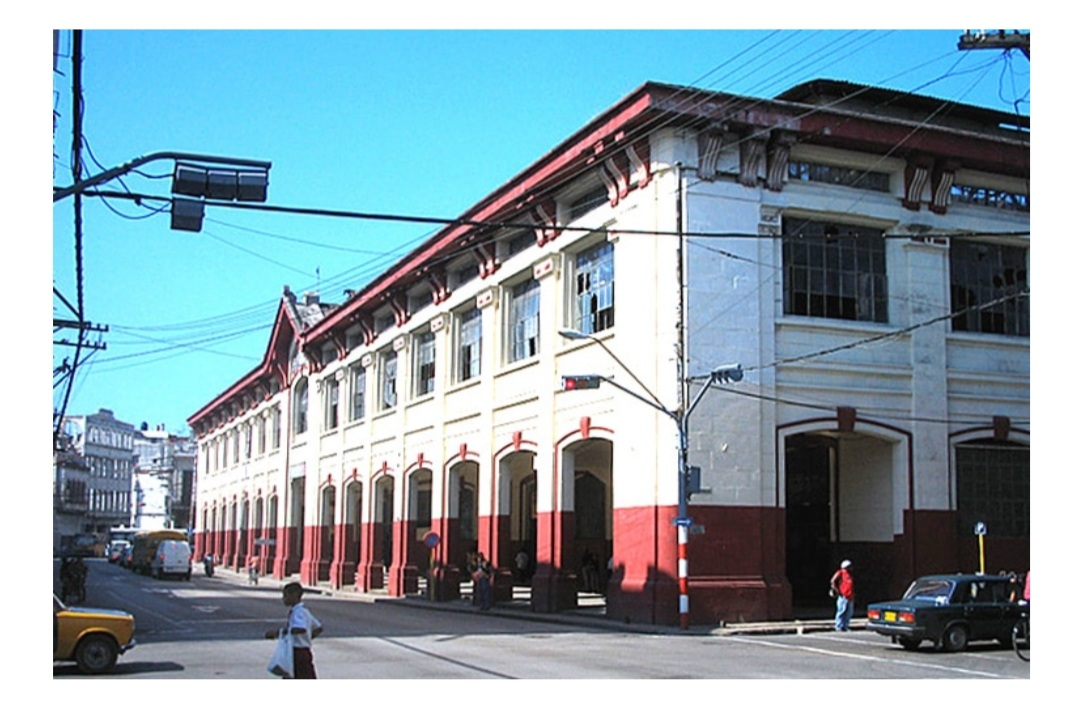
\includegraphics[width=0.7\linewidth]{cerro}
	\caption{}
	\label{fig:cerro}
\end{figure}



\subsection{Mapa de Localización:}

\begin{figure}
	\centering
	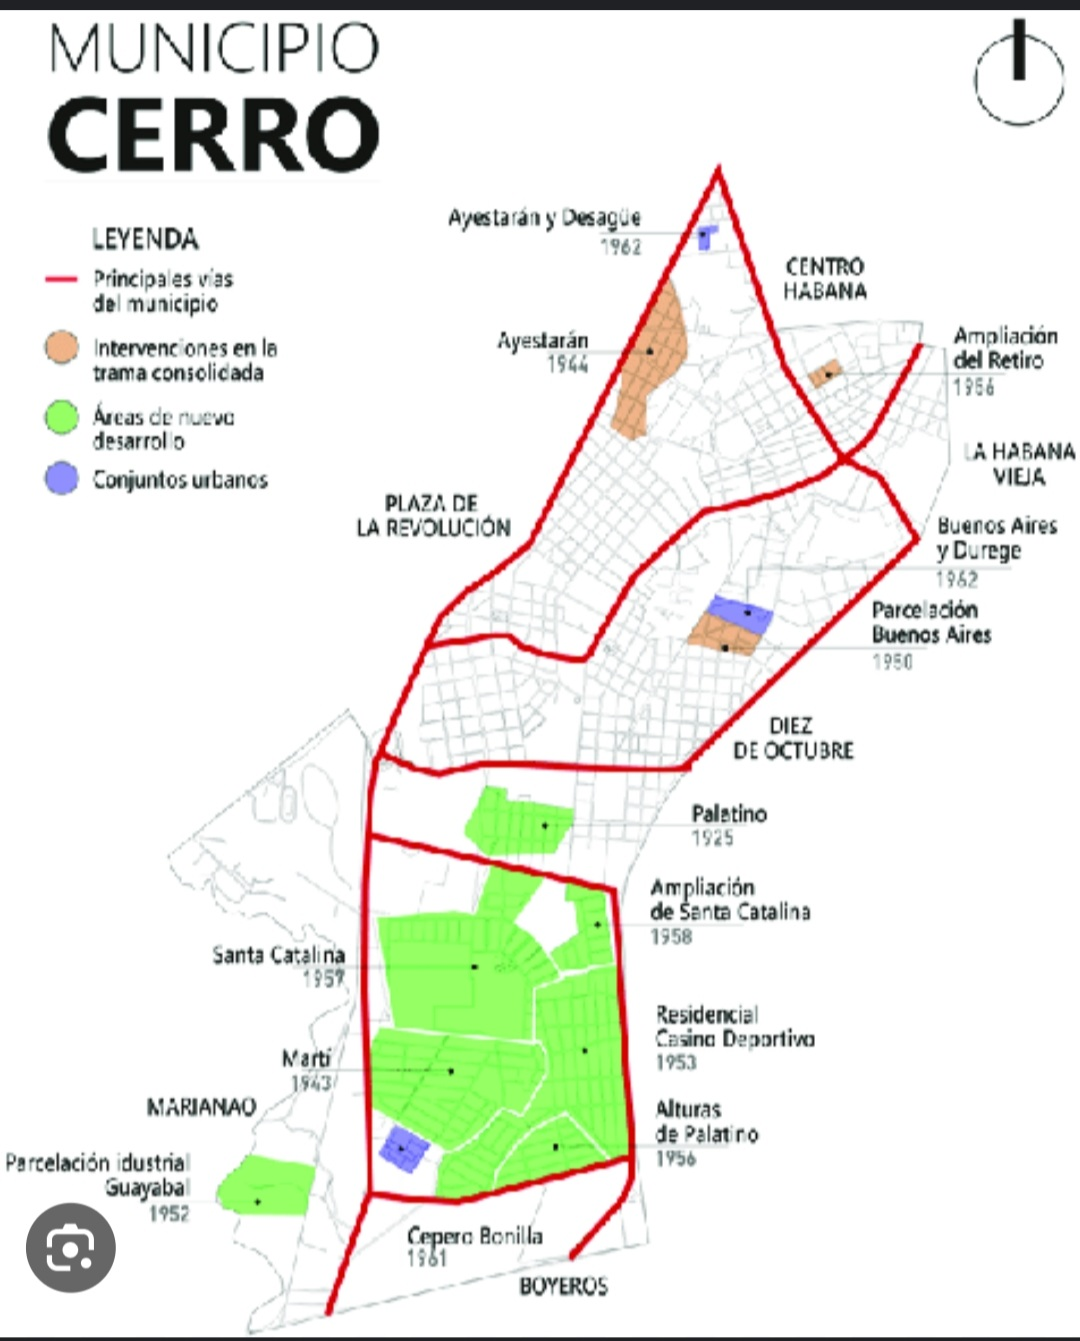
\includegraphics[width=0.4\linewidth]{mapa_cerro}
	\caption{}
	\label{fig:mapacerro}
\end{figure}




\onecolumn
\section{{\LARGE \underline{Desarrollo}}}

El análisis del proyecto se efectúa en un Jupyter Notebook que es una herramienta muy útil para realizar análisis de datos en ciencia de datos .Estos  notebooks permiten interactuar con los datos de manera interactiva , lo que significa que se pueden explorar los datos y realizar cambios en tiempo real , además de realizar visualizaciones y entender mejor su estructura .En ellos pueden agregar textos , imágenes y gráficos para explicar los hallazgos y conclusiones de las informaciones de manera clara y concisa por lo tanto representan la mejor opción para realizar este tipo de investigación.

\subsection{Importación del Json y Bibliotecas}

Luego se importa el json para trabajar con datos \underline{json.json} ya que es un formato de intercambio de datos ligero más fácil de leer y escribir y también se importan las bibliotecas de python como \underline{GeoPandas} que  proporciona una forma fácil de trabajar con datos geoespaciales utilizando Pandas DataFrames , \underline{NumPy} que se utiliza para trabajar con matrices y matrices multidimensionales proporcionando una forma fácil de realizar cálculos matemáticos complejos, \underline{Pandas} la cual se utiliza para trabajar con datos estructurados que provee una forma fácil de trabajar con datos tabulares utilizando DataFrames,\underline{Matplotlib} el cual se utiliza para crear gráficos y visualizaciones,\underline{Pyplot} es un módulo dentro de Matplotlib que proporciona una interfaz fácil de usar para crear gráficos y por último \underline{Plotly} se utiliza para crear gráficos interactivos y Express es un módulo dentro de Plotly que proporciona una interfaz fácil de usar para crear gráficos , también se importa el operador que es para organizar los valores.Luego el archivo json se abre para cargar los datos en la variable “dicc” esto  se hace porque el archivo json contiene datos estructurados que pueden ser procesados por el programa .Finalmente , todos elementos mencionados anteriormente  representan herramientas que facilitan el estudio.

\subsection{DataFrame:}

Además  se crea un \underline{DataFrame de Pandas} para representar los datos del dicionario de la cerveza, la cebolla y los refrescos y de esta manera tener una mejor trasparencia y facilidad para extraer los datos  y analizarlos .                                 

\section{Análisis de los datos de la cerveza}

\subsection{Precios}

Python cuenta con varias bibliotecas que facilitan los cálculos estadísticos como el módulo statistics que proporciona funciones para el cálculo de estadísticas descriptivas de datos numéricos y por ende es más fácil computar el promedio, la media, la mediana, la moda, entre otros.

También se cuenta con la representación gráfica para realizar una  visualización deductiva de los datos ,estas visualizaciones se pueden realizar con la biblioteca matplotlib y realizar el gráfico deseado ya sea un histograma, un gráfico de pastel,etc.

En este caso se analizo el precio de la cerveza , la misma tiene una variación de precios bastante amplia desde su precio mínimo que en este caso \$125 hasta su precio máximo que es \$300, además el precio más común de la cerveza es \$150 , esta información es de gran utilidad para los consumidores puesto que si un cliente tiene conocimiento del precio máximo , mínimo y más común del producto que quiere consumir , puede tomar decisiones informadas sobre cuánto está dispuesto a pagar por una cerveza en particular.

Asimismo se analizó el precio promedio de cada marca de cerveza donde la cerveza más cara es la Patronus que tiene un costo de \$250 ,y la más económica es la Cruz Campo con un precio de \$130 apróximadamente .La relación entre la marca de la cerveza y su precio aporta información valiosa sobre la demanda y la asequibilidad del producto , no obstante que una cerveza tenga un precio más bajo que otra no quiere decir que tenga una demanda mayor , simplemente puede deberse a que tiene menor distinción de marca , en este caso que la cerveza Cruz Campo o cualquiera de las cervezas importadas representadas  tengan un precio más económico que las cervezas del primer gráfico no quiere decir que sean más populares ni tenga mayor credibilidad que las demás puesto que la Patronus , cerveza procedente de Alemania cuesta \$250 ,este país es considerando el cuarto mayor exportador de cerveza otorgándole distinción y credibilidad a sus productos , también se destaca Holanda que importa la Hollandia Premium y la Holland Import que ambas tienen un precio que oscila entre \$150-\$200 y tienen alta demanda y credibilidad en el mercado.



\subsection{Países de Origen de la Cerveza}

Es de gran utilidad tener el conocimiento sobre los píses de origen de las cervezas que más predominan en el ayuntamiento , pues se llega a la conclusión precisa de que la mayoría de estas cervezas son importadas donde \underline{destacan Bélgica , Holanda y España} como los tres países con mayor porciento , lo que significa que son los países que más importan las cervezas que predominan en el municipio del Cerro . Las cervecerías holandesas son otras que han tenido mucho éxito internacionalmente ya que han logrado producir cerveza de buena calidad a un precio competitivo , en este caso predomina bastante como se menciona con anterioridad , representando un 18.4\%. Un dato interesante es el \% de los  Países Bajos , pues más de la mitad de la producción anual de cerveza de los Países Bajos está destinada a mercados de exportación , de hecho , son el segundo país mayor exportador de cerveza del mundo (después de México) y su \% no se encuentra entre los más altos , lo que lleva a la conclusión de que es un producto con una alta demanda o que no predomina mucho en la localidad .España es el segundo productor de cerveza en Europa, solo superado por Alemania , esto le permite tener una gran capacidad de producción , variedad de marcas y tipos de cerveza , ademas tiene una ventaja competitiva en el sector cervecero por su clima, su estilo de vida mediterráneo y su gastronomía , factores que hacen que la cerveza española sea apreciada por los consumidores extranjeros que buscan productos de calidad y sabor , por ello  se beneficia de la demanda internacional de cerveza y Cuba es uno de los paises  que mas demanda la cerveza española , debido al hecho de que el mismo  presenta escaza producción de cerveza por problemas de abastecimiento de materias primas y encuentra como alternativa la importación , pero el motivo real por el que se prefiere esta cerveza se debe a  los lazos históricos y culturales que unen a ambos países , además , esta cerveza como se explico con anterioridad  tiene una calidad y un sabor reconocidos internacionalmente , lo que la hace atractiva para los consumidores cubanos y por ello predomina en el pais , específicamente en el municipio del Cerro .

El código es bastante sencillo , pues creas una lista para introducir todos los países de procedencia de la cerveza y cuenta la cantidad de veces que aparece para luego hallar su porciento , y así representarlo en un gráfico de pastel.



\subsection{Volumen}

La cantidad de ml de una lata o botella de cerveza parece un aspecto insignificante , sin embargo es todo lo contrario , si se tiene en cuenta el precio de cada marca de cerveza , dato importante que se presento en observaciones anteriores , cuando comparas cada precio de esa cerveza con su cantidad de ml te podrás dar cuenta de que la cerveza mas económica no es la opción más factible en todas los casos , pues puede que tenga menor cantidad de ml , por ejemplo: una holland import de 330ml a 170  una holland import de 500ml a \$200, se podrás dar cuenta que no hay mucha diferencia en su precio pero sí en  la cuantidad  de ml que posee , entonces llegamos a la siguiente interrogante : ¿Qué es mas provechoso? claramente es mejor comprar una cerveza más cara con mayor cantidad de ml que una barata con menor , pues la diferencia de precios es mínima , no en todos los casos , se puede dar la situación de que la diferencia de precios sea exhuberante y pues no quede más solución que comprar las mas económica o dependiendo del gusto del consumidor según su economía.\\

El código se realiza fácilmente realizando una comprensión de listas de cada cantidad en ml y luego representarlo en un gráfico scatter, conocido como diagrama de dispersión.

\subsection{Porciento de alcohol}

El \% de alcohol de la cerveza es una medida de la cantidad de etanol que contiene , además este \% puede variar en dependencia según el país de procedencia , por ejemplo en algunos países europeos como Bélgica y Alemania , es común encontrar cervezas con mayor porciento , mientras que en otros países como en Estados Unidos , las cervezas suelen tener un \% de alcohol más bajo.Este porciento también puede estar relacionado con la tradición cervecera del país de origen y los ingredientes utilizados para elaborarla .Por ejemplo en Bélgica se utilizan levaduras especiales que pueden producir cervezas con un  alto contenido en alcohol , mientras que en México , las cervezas suelen tener un bajo contenido de alcohol debido a las altas temperaturas y la necesidad de mantenerse hidratado .Este análisis da respuesta a la pregunta inicial , teniendo en cuenta el hecho de que la mayoría de las cervezas presentes en el municipio son importadas como se puede observar en la tabla de datos de la cerveza inicial .Un dato es interesante es conocer que la cerveza con mayor porciento de alcohol , en este caso la 8.6\% que curiosamente su nombre coincide con su \% de alcohol.\\

Al igual que en los casos anteriores el código es bastante sencillo si se utiliza una compresión de listas o la biblioteca Pandas que simplifica los códigos.


\subsection{Envase}

Se crea un dicionario vacío y luego con un for se recorre el diccionario cerveza y cuenta la cantidad de veces que aparece cada tipo de envase , donde el envase de lata que predomina por encima encima del envase de botella , es un dato de conocimiento público , pero el cual tenemos bases para fomentar como se explica a continuación.\\

La mayoría de las cervezas que se encuentra actualmente en nuestro país , en este caso en el municipio del Cerro , pertenecen a países extranjeros , lo que deja claro que se tienen  muy pocas cervezas nacionales en el país  y  la mayoría son importadas .Esta situación puede deberse a varios factores , uno de ellos puede ser que la cerveza en lata es el envase preferido en la mayoría de  los casos para la exportación de esta por la facilidad de transporte , ya que son más ligeras y resistentes que los envases de vidrio  , también son mas fáciles de almacenar , apilar y manipular en grandes cantidades , son menos propensas a romperse  y no permiten la entrada de luz , lo que puede danar el sabor de la cerveza .Es más fácil y económico poducir latas que botellas de vidrio , y esto puede influir en el costo total  del producto  y en su atractivo en el mercado , provocando exhuberantes precios de la cerveza , pues entre más caro cuesta el tipo de envase del producto teniendo en cuenta también el costo de los ingredientes para su producción la cerveza tomaría un precio mayor , convirtiendose en un lujo su consumo , por ende la mayoría de los países exportan cerveza en lata debido a su facilidad de transporte , almacenamiento , resistencia y costo .

El otro factor se encuentra relacionado a las ventajas o desventajas que el tipo de envase puede provocar como por ejemplo en su sabor y su aroma.\\

\begin{enumerate}
	\item{La exposición al oxígeno puede alterar el sabor y el aroma de la cerveza .Las botellas de vidrio son mejores para mantener la frescura de la cerveza , ya que el vidrio es impermeable al oxígeno}
	\item{La luz UV también puede afectar negativamente la calidad de la cerveza .Las botellas de vidrio oscuro o las latas son más efectivas para bloquear la luz}
	\item{Algunos envases pueden mantener mejor la temperatura de la cerveza,lo que podría influir en su sabor .Las latas son excelentes para mantener la ceveza fría , mientras que las botellas de vidrio pueden mantener mejor temperatura a largo plazo}
	\item{El transporte es un aspecto esencial,el tipo de envase puede afectar la portabilidad y la facilidad de transporte de la cerveza.Las latas son mas ligeras y fáciles detransportar, mientras que las botellas de vidrio pueden ser más frágiles y pesadas}.
\end{enumerate}.\\
	
En resumen,el tipo de envase de la cerveza puede influir en calidad,sabor,aroma,temperatura y facilidad de transporte .


\subsection{Análisis de los datos de la cebolla}

Al igual que para el análisis de la cerveza se utiliza el módulo statistics de python para calcular el precio promedio de la cebolla, el precio más común, es decir la moda,también se crea comprensión de listas junto con un for para determinar la cantidad de cebollas que se venden en ristras y las que se venden en libras 



El objetivo de este análisis es comparar los precios promedios entre la cebolla blanca y la cebolla morada para determinar si hay una diferencia significativa entre los precios de los dos tipos de cebolla  , además se evidencia que el precio promedio más alto es el de la cebolla morada pues es \$280.Esto puede ser útil para los agricultores y los minoristas que venden cebollas, ya que pueden ajustar sus precios en consecuencia . Además , representa un dato de utilidad  para los consumidores , quienes pueden  comparar los precios de diferentes tipos de cebolla para ayudarles a tomar decisiones sobre qué tipo de cebolla comprar según sus necesidades y economía .\\


El dato del precio más común de cada tipo de cebolla se aprovecha para hacer comparaciones de los distintos precios en diferenes lugares y saber si es o no un precio razonable con la oferta de mercado .\\

La cebolla blanca es más común que la cebolla morada , ambas tienen diferentes propiedades nutricionales. La cebolla morada es más rica en antioxidantes, ya que contiene un mayor número de antocianinas , además posee más quercetina, la cual previene tumores malignos y favorece la producción de glóbulos blancos , lo que justfica su escazes pues es un producto que debido a sus propiedades tiene mayor demanda en el mercado.\\

Todo estos estos análisis se respaldan con ayuda de gráficos para realizar una visualización más deductiva de este estudio y así el lector obtenga un efectue una mejor comprensión del tema.En estos gráficos predomina el gráfico de barra .\\

Es importante destacar que gracias a la utilización de estos códigos se realizan cálculos efectivos que permiten llegan a conclusiones más certeras como en el análisis siguiente:

La cebolla en libra es más abundante que la venta de cebolla en ristra , a qué se debe ? Es de conocedor social que la cebolla se vende más en libra que en ristra debido a que la libra es una medida de peso , más precisa y fácil de transportar y la ristra es una medida de cantidad , su transportación es más compleja y mucho más difícil de almacenar , asimismo se puede sostener la hipótesis que da más negocio su venta en libra pues su precio es más económico y dispones de comprar solo la cantidad necesaria para el consumo , ya que en ristra además de su alto valor , el cual no todos los individuos se pueden dar el lujo de pagar , se comercia por cantidad corriendo el riesgo de que se pueda deteriorar , ya que cada persona tiene un método de ahorro diferente y al ser más cara y mayor cantidad lo más lógico es que la tiendan a economizar lo que puede provocar su deterioro.\\

Otro aspecto es que en el municipio del Cerro predomina la escazes de carretilleros y prevalecen los agros , aunque en el próximo análisis quedará claro que realmente en municipio  Cerro se puede encontrar tanto escazes de carretilleros como de agros .

\subsection{Análisis de los datos de los refrescos}

Al analizar el precio promedio de cada marca de refresco y representarlos graficamente se observa una variedad de precios bastante amplia .La explicación a este fenómeno es sencilla , la mayoría de los refrescos tiene características específicas como la cantidad en ml , el azúcar , las calorías , sabor suave o sabor intenso , de gas o sin gas , estos son aspectos que se tienen en cuenta para los ingredientes de su producción , que influye en la economía , al igual que la marca del refresco que también incide , existen marcas más reconocidas que otras y viceversa , en este caso el refresco mate de origen cubano presenta el precio promedio de mayor categoría , un poco contradictorio ya que el refresco de precio mínimo es el de naranja , también de origen cubano .
¿Cómo se puede fomentar esta hipótesis?
Para responder esta pregunta se debe analizar todos los factores que influyen en el precio de un producto como se explicó con anterioridad , puede que los ingredientes del refrescos mate sean más caros o más difíciles de conseguir que los del frised de naranja ,que son refrescos de marca importada , además del proceso de producción que se lleva a cabo , donde existe la posibilidad de que uno sea más complejo que otro , pero el factor fundamental , el sustento de este planteamiento es la demanda del mercado , este refresco es considerado  una de las bebidas más refrescante y distintivas de Cuba , que en los tiempo actuales aparece muy poco en el mercado y cuando lo hace no dura mucho tiempo en él , pues tiene una oferta bastante buena , ese es uno de los motivos del precio exhuberante del refresco mate , pues es una cuestión de oferta y demanda , mientras más célebres y escazos suelen ser algunos productos , existe mayor inferencia en su excesivo precio .En cambio el frised de naranja es un producto que no lleva mucho tiempo en el mercado , como este predominan muchos refrescos importados que se venden bien por su módico precio , sabor o frescura del mismo , pero no por su fama o credibidad .\\

El precio más común de los refrescos es \$150 , dato que además  coincide con la moda .Esta información ayuda en la toma de decisiones , pues tienes el conocimiento de si estas obteniendo una buena oferta del producto o estas pagando de más , teniendo la posibilidad de hacer una comparación con el precio del mismo producto en diferentes lugares y optar por la opción más viable para tu consumo . Además si eres propietario de un negocio  puede ayudarte a planificar mejor tus estrategias de precios y marketing , si sabes cuánto están dispuesto a pagar tus clientes por un producto en particular , puedes ajustar tus precios para maximizar tus ganancias y atraer más clientela .\\

Los refrescos en lata predominan más que los refrescos en pomo , pero eso no quiere decir que las personas tengan más preferencia por uno que por otros , eso depende más de sus gustos personales y de las situaciones en las que se encuentre el refresco .
No obstante al igual que en el caso de cerveza el tema del envase tiene sus ventajas y desventajas :
Las latas son fáciles de transportar y herméticas lo que ayuda a mantener el gas y el sabor del refresco , además son reciclables y tienen una huella de carbono menor que los pomos de plástico pero el sabor del refresco puede verse afectado por el metal de la lata , además de ser mas difíles de abrir y beber directamente de ellas .
En cambio los pomos de plástico son fáciles de abrir y beber directmente de ellos , el sabor del refresco puede ser más fresco y natural ya que el plástico no afecta tanto el sabor como el metal de la lata pero pueden ser más pesadas y voluminosas que las latas , lo que las hace menos fáviles de transportar y almacenar , también son menos herméticas que lo que afecta la frescura y el gas del refresco .
En conclusión la elección de un refresco en dependencia de su envase se basa más en preferencias personal y según la situación , pues si andas apurado o en un estado incomodo resulta más factible un refresco en pomo ya que lo cierras con la tapa y listo , no corres el riesgo de que se bote ni nada parecido , en cambio si fuera una lata si corres ese riesgo , además los resultados de la cantidad de envases de cada tipo estan bastante relacionados con la hipótesis de que el refresco que más se consume es en envase de pomos de plástico.\\

El refresco que más predomina en las cafetrías es el pepsi cola , información que se profundizará más adelante.\\


Cada producto , en este caso los refrescos , contiene en la etiqueta de su envase la información sobre la cantidad de energía y nutrientes por 100  gramos o 100 mililitros del alimento , dicha información es obligatoria en el etiquetado nutricional .La calidad nutricional de un alimento , su valor nutritivo , hace referencia a la contribución de dicho alimento al aporte total de nutrientes de la dieta , es decir , los nutrientes que nos aporta y su biodisponibilidad , refiriéndose a la composición en términos de energía y nutrientes .Este valor nutricional se puede determinar a través del cálculo de las kilocalorías proporcionadas por los nutrientes que contienen energía , en otras palabras , de las kilocalorías que aportan las proteínas , los hidratos de carbono , las grasas y el alcohol .La realidad es que este aspecto es muy importante , ya que conocer la información nutricional de un producto permite a cualquier consumidor priorizar los alimentos más nutritivos y así mantener una alimentación sana y equilibrida cada vez mayor , además facilita la selección apropiada del producto de acuerdo a las necesidades y condiciones de salud de cada persona.\\


El país que mayor cantidad de refrescos importa a Cuba es Estados Unidos , ¿A qué se debe este fenómeno?.\\


\underline{artículo:} La industria de refrescos a nivel mundial - Datos estadísticos.statista

Estados Unidos domina el mercado :.\\

Ahora bien , es de sobra conocido que si hay un país que lidera el sector ese es Estados Unidos .Tan solo en 2021, ingresó casi 311.000 millones de dólares gracias a los refrescos, quintuplicando así la cantidad facturada por Japón, en segundo lugar .Pero estos datos no son más que el reflejo de la alta demanda de este producto que existe dentro de sus fronteras .Los cerca de 225,5 litros de gaseosas y sus diferentes variedades ingeridos de media por cada ciudadano en 2021 convierten al Tío Sam en el país con mayor volumen de consumo per cápita a nivel global .Ante esta situación , no sorprende que a día de hoy siga manteniéndose como el máximo consumidor de bebidas no alcohólicas del mundo , ni que haya sido en su territorio donde nacieron dos de los máximos referentes de la industria mundial.
Coca-Cola y Pepsi , la eterna competencia
Y esos dos nombres no son otros que The Coca-Cola Company y PepsiCo .Aunque ambas deben su origen a la farmacia–dos profesionales de dicha disciplina fueron los creadores de las fórmulas que hoy son su factor diferenciador-la primera de ellas nació alrededor de una década antes que su histórico rival .Este tiempo sin competidores directos ayudó a la multinacional dirigida por James Quincey a posicionarse positivamente entre un público que deseaba una bebida no alcohólica con cuerpo y de sabor agradable .La buena acogida no ha cesado desde entonces , en especial , en lo que respecta a su marca insignia , Coca-Cola , que continúa alzándose como la más valiosa del mundo dentro de las “bebidas vírgenes” a una diferencia de más de 70.000 millones de Red Bull , en segundo puesto .Esta ligera desventaja inicial no ha impedido , sin embargo , que PepsiCo se haga con una clientela fiel , que el posterior lanzamiento de opciones sin gas como el té helado Lipton no ha hecho sino afianzar .Además , en términos financieros , la empresa con sede en Nueva York no tiene nada que envidiar a la firma georgiana .Y es que las ventas de ambos gigantes nunca bajan de los 30.000 millones de dólares , colándose siempre entre las diez primeras compañías dentro del sector de bebidas sin alcohol. 

Este artículo explica en detalle como este país se ha convertido en una de las potencias más exportadoras de refresco , hecho que justifica que sea el país de origen de las marcas de refrescos que más predominan en el municipio , especifícamente la marca pepsi cola que como se analizó anteriormente es la marca moda de todos los tipos de refrescos , acontecimiento que no implica que sea el producto que  más  se consume , sino que tiene un precio bastante módico  como se puede observar en la tabla de las marcas de los refrescos con su precio correspondiente.
Un dato sugestivo es el 7.4\% de cantidad de marcas de refrescos que no le corresponden a ningún país , sería null por eso es que no sale ningún país de procedencia , pues los refrescos de marca Luni tiene procedencia desconocida , además según las estadísticas de la cantidad de refrescos de cada marca presente solo se encuentra 2 veces , es decir que no es una marca influyente en el territorio o muy poco consumida.\\


\newpage
\url{https://es.statista.com/temas/9705/la-industria-de-refrescos-en-el-mundo/}

\footnote{link con la informción extraída}

\newpage
\section{{\LARGE \underline{Conclusiones}}}

Según los análisis realizados de cada producto en el desarrollo del notebook , es evidente que hay factores comunes de cada producto que tienen gran utilidad , tener conocimientos acerca de:

\begin{itemize}
	\item{la variación del precio de cada uno de ellos}
	\item{el precio promedio}
	\item{las marcas}
	\item{la cantidad de ml}
	\item{los beneficios de cada cebolla}
\end{itemize}
	
Así sucesivamente la relación  entre todos los aspectos analizados con anterioridad , se concluye que la  mayoría de las cervezas y refrescos que predominan en el país son los importados , y que el precio de cada uno de ucellos no tiene mucha relación con su demanda en el mercado , que algunos de los países de origen que exportan estas marcas coinciden y se llega al resultado de que tienen una pequeña relación , además la escasez de cebollas y agros presentes en el municipio es un tema delicado que deberían tratar de solucionar por necesidad  , y en beneficio de la población.


\newpage
\tableofcontents


\end{document}

